\documentclass{beamer}

\usepackage{graphicx,hyperref,udesc,url}
\usepackage[brazilian]{babel}
\usepackage[utf8]{inputenc}
\usepackage[T1]{fontenc}
\usepackage{booktabs}
\usepackage{ragged2e}
\usepackage{times}


\title{Exemplo de apr de slides}
\subtitle{Um exemplo 2015}

\author{Nicolas P. Lane, Autor2\\
    {\small \url{nicolaspeterla@hotmail.com}} \\ 
    {\small \url{email@author2.com}}
}

\institute[UDESC]{
    Departamento de Ci\^encia da Computa\c{c}\~ao \\
    Centro de Ci\^encias e Tecnol\'ogicas\\
    Universidade do Estado de Santa Catarina
}

\begin{document}
%%%%%%%%%%%%%%%%%%%%%%%%%%%%%%
\frame[shrink]{
    \titlepage
}
%%%%%%%%%%%%%%%%%%%%%%%%%%%%%%
%Usar shrink no [] se precisar colocar mais seções e subseções e não dispor de mais espaço
\frame{
    \frametitle{Sum\'ario}
    \tableofcontents
}
%%%%%%%%%%%%%%%%%%%%%%%%%%%%%%
\section{Introdu\c{c}\~ao}
%%%%%%%%%%%%%%%%%%%%%%%%%%%%%%
\frame[shrink]{
    \begin{figure}
        \centering
        
\includegraphics[width = 0.5\textwidth]{figures/Subversion}%Usar um diretório a partir do projeto: diretorioA/nomeDoArquivo.png ou jpg
    \end{figure}

    \frametitle{Hist\'oria}
    \begin{itemize}
        \item{ CollabNet fundou em 2000}
        \item{ Foi aceito em uma incubadora do grupo Apache em 2009}
    \end{itemize}
}
%%%%%%%%%%%%%%%%%%%%%%%%%%%%%%
\frame{
    \frametitle{Motiva\c{c}\~ao}
    \begin{itemize}
        \item{Competir com o CVS}
        \item{Proposta Livre}
        \item{Corrigir v\'arios problemas do CVS}
        \item{Novas funcionalidades}
    \end{itemize}
}
%%%%%%%%%%%%%%%%%%%%%%%%%%%%%%
\frame{
    \frametitle{Quem usa}
    \begin{itemize}
        \item{Comunidade de Software Livre}
        \item{Grupo Apache}
        \item{Google}
        \item{Apple}
    \end{itemize}
}
%%%%%%%%%%%%%%%%%%%%%%%%%%%%%
\section{Caracter\'isticas em Particular}
%%%%%%%%%%%%%%%%%%%%%%%%%%%%%
\begin{frame}
    \frametitle{Pontos Importantes}
    \begin{itemize}
        \item{Versionamento de diretórios}
        \item{Histórico de versões efetivo}
        \item{Manipulação consistente de dados}
        \item{Commit \'atomico}
        \item{Versionamento de metadados}
        \item{Ramificações e rotulagem eficiente}
        \item{Hackability}
    \end{itemize}
\end{frame}
%%%%%%%%%%%%%%%%%%%%%%%%%%%%%%
\frame{
    \frametitle{Reposit\'orio}
    \begin{columns}

        \begin{column}{.555555\textwidth}
            \begin{block}{Arquitetura}
                \begin{columns}
                    \begin{column}{.5\textwidth}
                        \begin{itemize}
                            \item Cliente-Servidor
                        \end{itemize}
                    \end{column}
                    \begin{column}{.5\textwidth}
                        \begin{figure}
                            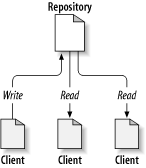
\includegraphics[width = 0.7\textwidth]{figures/repositorio}
                        \end{figure}
                    \end{column}
                \end{columns}
            \end{block}
        \end{column}

        \begin{column}{.5\textwidth}
            \begin{block}{Estrutura de arquivos}
                \begin{columns}
                    \begin{column}{.5\textwidth}
                        \begin{itemize}
                            \item \'Arvore de arquivos
                        \end{itemize}
                    \end{column}
                    \begin{column}{.5\textwidth}
                        \begin{figure}
                            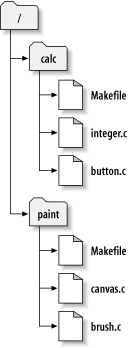
\includegraphics[width = 0.7\textwidth]{figures/arquivos}
                        \end{figure}
                    \end{column}
                \end{columns}
            \end{block}
        \end{column}
    \end{columns}
}
%%%%%%%%%%%%%%%%%%%%%%%%%%%%%
\section{Conceitos B\'asicos}
%%%%%%%%%%%%%%%%%%%%%%%%%%%%%
\frame{
    \frametitle{Reposit\'orio 2}

    \begin{columns}
        \begin{column}{.5\textwidth}
            \begin{itemize}
                \item{Simples cole\c{c}\~ao de arquivos}
                \item{Centralizado}
                \item{Working copy - Os desenvolvedores trabalham com copias locais}
            \end{itemize}
        \end{column}
        \begin{column}{.5\textwidth}
            \begin{block}{Pastas}
                \begin{enumerate}
                    \item{.svn}
                    \item{trunk}
                    \item{branches}
                    \item{tags}
                \end{enumerate}
            \end{block}
        \end{column}
    \end{columns}
}
%%%%%%%%%%%%%%%%%%%%%%%%%%%%
\frame{
    \frametitle{Revis\~oes}
    \begin{columns}
        \begin{column}{.5\textwidth}
            \begin{itemize}
                \item{Estado do reposit\'orio}
                \item{Uma maneira de voltar no tempo}
                \item{Podem ser marcado com Tags}
            \end{itemize}
        \end{column}
        \begin{column}{.5\textwidth}
            \begin{figure}
                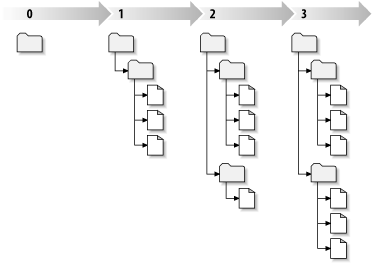
\includegraphics[width=1.0\textwidth]{figures/revisao}
            \end{figure}
        \end{column}
    \end{columns}
}
%%%%%%%%%%%%%%%%%%%%%%%%%%%
\frame{
    \frametitle{Modificando Arquivos}
    \begin{block}{O problema do compartilhamento de arquivo}
        \begin{columns}
            \begin{column}{.5\textwidth}
                \begin{itemize}
                    \item{Sobrescrever}
                \end{itemize}
            \end{column}
            \begin{column}{.5\textwidth}
                \begin{figure}
                    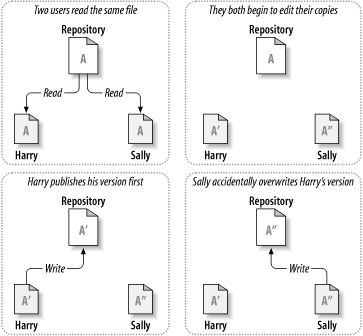
\includegraphics[width=0.9\textwidth]{figures/problem}
                \end{figure}
            \end{column}
        \end{columns}
    \end{block}
}
%%%%%%%%%%%%%%%%%%%%%%
\section{Refer\^encias}
%%%%%%%%%%%%%%%%%%%%%%
\frame{
    \frametitle{Refer\^encias}

    \begin{itemize}
        \item{SVN Book - http://svnbook.red-bean.com/}
        \item{SVN Tutorial - http://www.tutorialspoint.com/svn/}
    \end{itemize}
}
%%%%%%%%%%%%%%%%%%%%%%%
\end{document}
